\documentclass[preprint,12pt]{article}
\usepackage[T1]{fontenc}
\usepackage{graphicx}
\usepackage{amsmath}
\usepackage{verbatim}

\newcommand{\ch}{\v{c}}
\newcommand{\tj}{\'c}
\newcommand{\ndi}{\chi_m^e}
\newcommand{\sd}{\chi_\Sigma^e}
\newcommand{\E}{\mathcal{E}}

\DeclareMathOperator{\MSE}{MSE}
\DeclareMathOperator{\MAE}{MAE}
\DeclareMathOperator{\avg}{avg}

\begin{document}

\begin{titlepage}
\title{
	{Proposition of new system for chess problem solvers' ratings}
	}
\author{Bojan Vu\ch kovi\tj}
\end{titlepage}


%\begin{abstract}
%\end{abstract}


\maketitle

\section{Introduction}

Let $R_i$ denote rating of the $i$-th solver in the tournament table,
and let $S_i$ denote his score, for every $i \in \{1,\dots,n\}$.
Next, let
\begin{equation}\label{mu_r}
\mu_r = \frac{1}{n}\sum_{i=1}^n R_i
\end{equation}
be the average rating, and let
\begin{equation}\label{mu_s}
\mu_s = \frac{1}{n}\sum_{i=1}^n S_i
\end{equation}
be the average score of solvers with rating.
According to the current rules, solvers' ratings change is
calculated with the following formula:
$$\E_i = (R_i-1600) \times \frac{\mu_s}{\mu_r-1600},$$
where $\E_i$ denotes the expected result of a solver with rating $R_i$.
The formula above is based on the assumption that results
and ratings of solvers are evenly distributed over the full range of possibilities.
This leads to a frequent necessity for corrections of the expected scores,
using the following formula:
\begin{equation}\label{old_corrected_system}
\E'_i = \mu_s +
(\E_i-\mu_s) \times \frac{S_{\max} - \mu_s}{E_{\max}-\mu_s},
\end{equation}
where $S_{\max} = \max_i S_i$, while $E_{\max} = \max_i E_i$.

In this note, a new system for calculating expected result of
rated solvers is proposed.
This system is based on the assumption that solvers' ratings,
as well as their scores on problem solving competitions,
are distributed according the normal distribution.
Proposed system could be applied to current rating list of solvers,
without any need for modifications of solvers' ratings.
It is also well suited for calculation of rating performance
that could be used as a measure of introducing rating for unrated solvers.

\section{Proposition}

Normal distribution is one of the most important distributions in
probability theory, and it is frequently used in many fields of scientific research.
System proposed here is basically a simple transformation
from distribution of solvers' ratings
to distribution of their scores.

Calculations start from a table of chess solving competition
containing informations about current rating and score of
every solver in the competition.
We are calculating expected score for every solver,
as well as his/hers rating performance.
For solvers who are new to solving competitions and do not possess rating,
calculated rating performance may be used for establishing initial rating.

First, we exclude results of all unrated solvers from the tournament table.
Now, let us assume that there are scores and ratings of $n$ solvers in the table.
Let
\begin{equation}\label{sigma_r}
\sigma_r = \sqrt{\frac{\sum_{i=1}^n (R_i - \mu_r)^2}{n}}
\end{equation}
be the standard deviation of solvers' ratings, and let
\begin{equation}\label{sigma_s}
\sigma_s = \sqrt{\frac{\sum_{i=1}^n (S_i - \mu_s)^2}{n}}
\end{equation}
be the standard deviation of rated solvers' scores,
where $\mu_r$ and $\mu_s$ are given by
\eqref{mu_r} and \eqref{mu_s}, respectively.

For calculation of the expected score $E_i$ of a rated solver with rating $R_i$,
we propose formula:
\begin{equation}\label{expected_res}
E_i = (R_i-\mu_r)\times \frac{\sigma_s}{\sigma_r}+\mu_s.
\end{equation}
On the other hand, for calculation of the rating performance $P_i$ for any solver
(including those without rating) with $S_i$ points, there is an analogue formula:
\begin{equation}
P_i = (S_i-\mu_s)\times \frac{\sigma_r}{\sigma_s}+\mu_r.
\end{equation}

Let $S_{\max}$ be the maximum number of points obtainable in the given competition.
Let $E_{\max}$ and $E_{\min}$ be the maximum and the minimum
number of points expected by a solver,
calculated by formula~\eqref{expected_res}.
In other words, $E_{\max}$ and $E_{\min}$ are the expected results
of the highest and lowest rated solver, respectively.
Let 
\begin{equation}
c = \max(E_{\max}-S_{\max}, -E_{\min}, 0).
\end{equation}
When the average score in a competition is very high or very low,
it is possible that expected score of some solvers
is more than $S_{\max}$ or less then $0$.
For that reason, we make a following correction of the expected scores:
\begin{equation}
E'_i = \min (E_{\max}-c, \max(E_i, E_{\min}+c)).
\end{equation}

That means that a solver may still lose rating even if he
makes a better score of all of other participants, but he may not lose
rating if he makes a perfect score.
The same holds for competitions in chess "over the board", where
a player may win a tournament and still lose rating points
if his opponents had much lower rating,
but he may not lose rating if he wins all games.

In rare cases, there might be a small difference in values of
$\sum_i E_i$ and $\sum_i E'_i$.
To keep the rating change of the competition equal to $0$,
we propose the final correction of expected results:
\begin{equation}
E''_i = E'_i + \avg_i(E_i-E'_i),
\end{equation}
with
\begin{equation}
\avg_i(E_i-E'_i) = \frac{\sum_i^n E_i - \sum_i^n E'_i}{n},
\end{equation}
where $n$ is the number of rated solvers in competition.

Rating change $C_i$ for a rated solver with rating $R_i$ and score $S_i$ 
is now calculated with:
\begin{equation}
C_i = (S_i - E''_i)\times KT,
\end{equation}

where $KT$ is the standard tournament coefficient (between $1$ to $4$).

An important property of the proposed system is that
a sum of rating change of all solvers is always equal to $0$.
This means that the rating system would not suffer of inflation or deflation
from its implementation.

\section{Comparison of the proposed and current rating change system}

\subsection{Calculation comparison}

Probably the best way to understand how rating systems, proposed and current one,
are calculating expected results is to take a look at charts
produced from some competition results.

\begin{figure}[h]
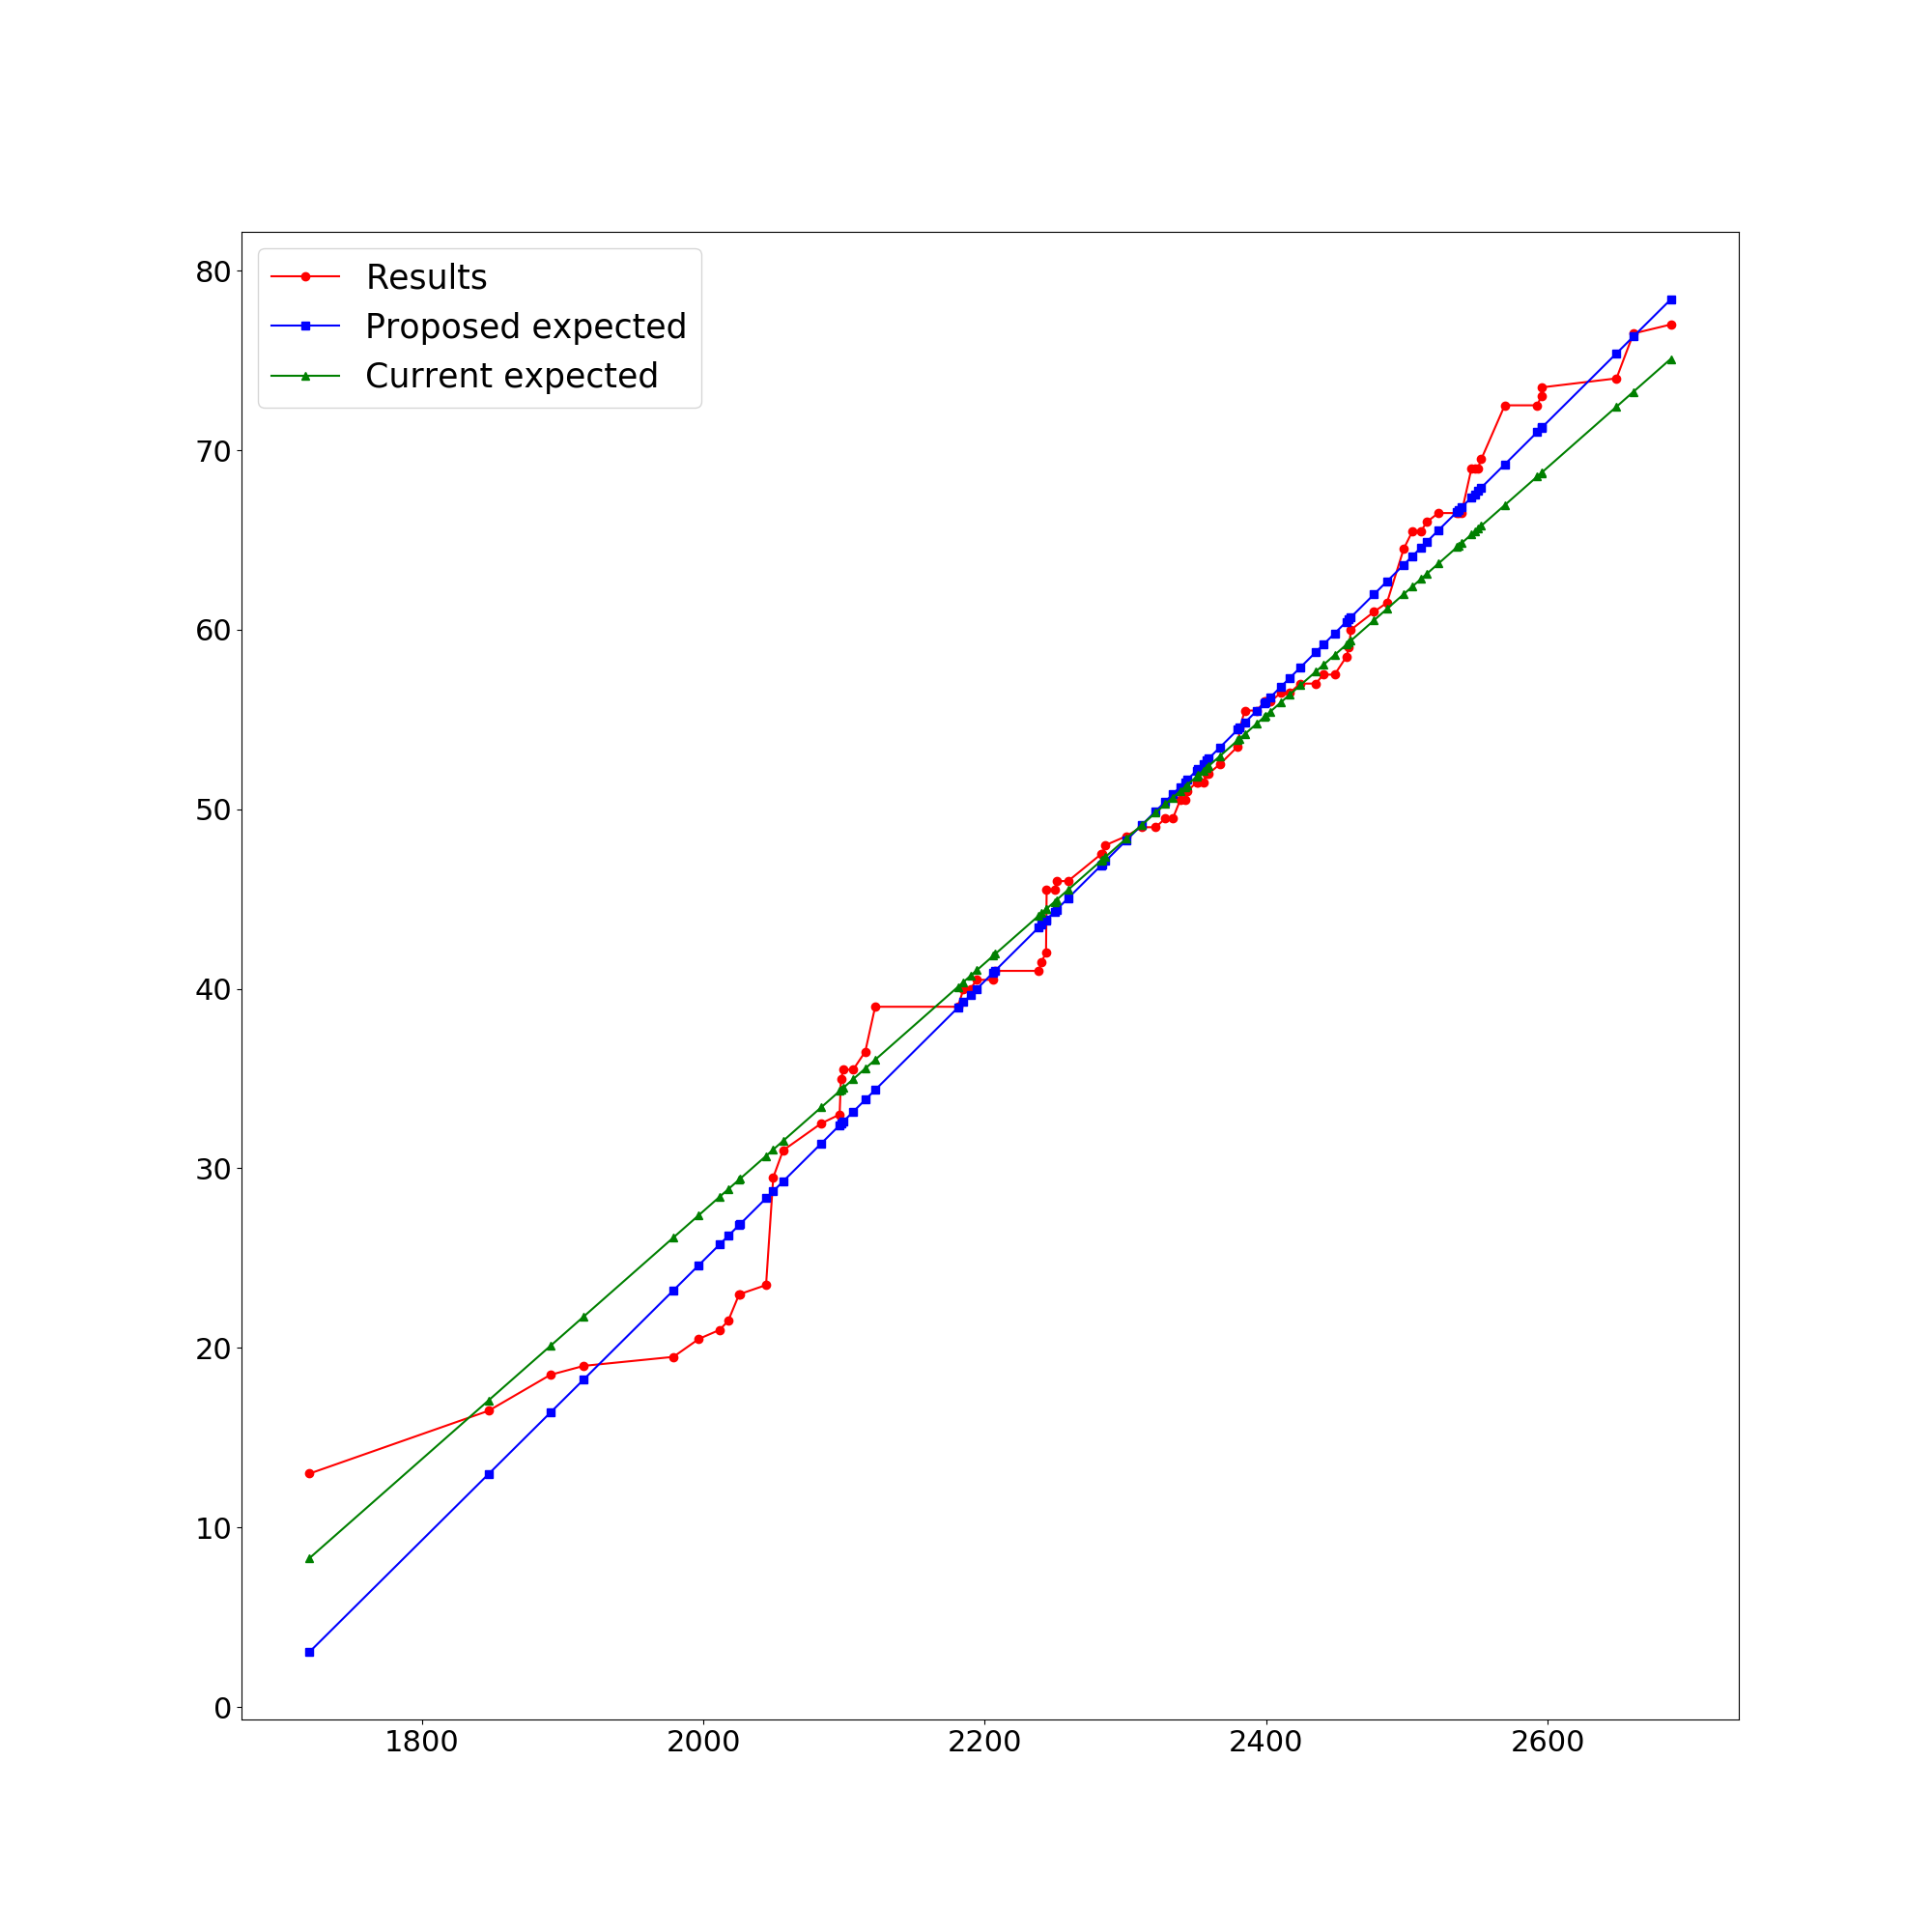
\includegraphics[width=1.0\linewidth]
{Dresden_points}\caption{WCSC 2017 points}
\label{dresden_2017}
\end{figure}

Table~\ref{dresden_2017} shows relationship between the solvers rating and
expected results is Dresden 2017 WCSC.

\subsubsection{Current system}

According to the current rating system,
expected results are calculated by taking into account the
average rating $\mu_r$ and average score $\mu_s$ of solvers in competition.
Expected result of every competitor
is determined by the line that goes through points
$(\mu_r, \mu_s)$ and $(1600, 0)$.
That is, the expected result of a solver with rating $1600$ is $0$,
while the expected result of a solver with rating $\mu_r$ is $\mu_s$.
Expected results of other solvers are calculated to match points on this line.
For WCSC 2017 expected results are presented by a green line in Figure~\ref{dresden_2017}.

In case when the expected result of a solver with the highest rating $R_h$
is greater than the result of the solver with highest score $S_h$,
the following corrections are made. Instead with the point $(1600, 0)$,
expected results are determined by the point $(R_h, S_h)$, that is
by the line that goes through points $(\mu_r, \mu_s)$ and $(R_h, S_h)$.
For Israel open 2017 this correction is presented by a cyan line in Figure~\ref{israel_2017}.

\subsubsection{Proposed system}

Calculation of the expected results is currently somewhat arbitrary,
and the proposed system deals with this problem.
Like in the current rating system, the system proposed here
also evaluates expected result according
a line that passes through point $(\mu_r, \mu_s)$.
The difference is that it also takes into account distribution of
ratings and points of solvers, and according the proportion of
$\sigma_r$ and $\sigma_s$, given by~\eqref{sigma_r} and \eqref{sigma_s},
calculates slope of this line.
For WCSC 2017 expected results from proposed system
are presented by a blue line in Figure~\ref{dresden_2017}.

In some cases, when the expected result of some of the solvers is
more than the maximum possible score, or less than $0$,
corrections are made so that no one would lose rating
after solving all problems, or gain rating after making $0$ points.
These correction are made so that the expected results are symmetrical
around the point $(\mu_r, \mu_s)$.
Figure~\ref{israel_2017} shows expected results in Israel open 2017.
This is a case where there has to be made corrections on both the current
and the proposed system, since the average score of solvers was high ($36.82$),
while the maximum achievable score was $60$ points.

\begin{figure}[h]
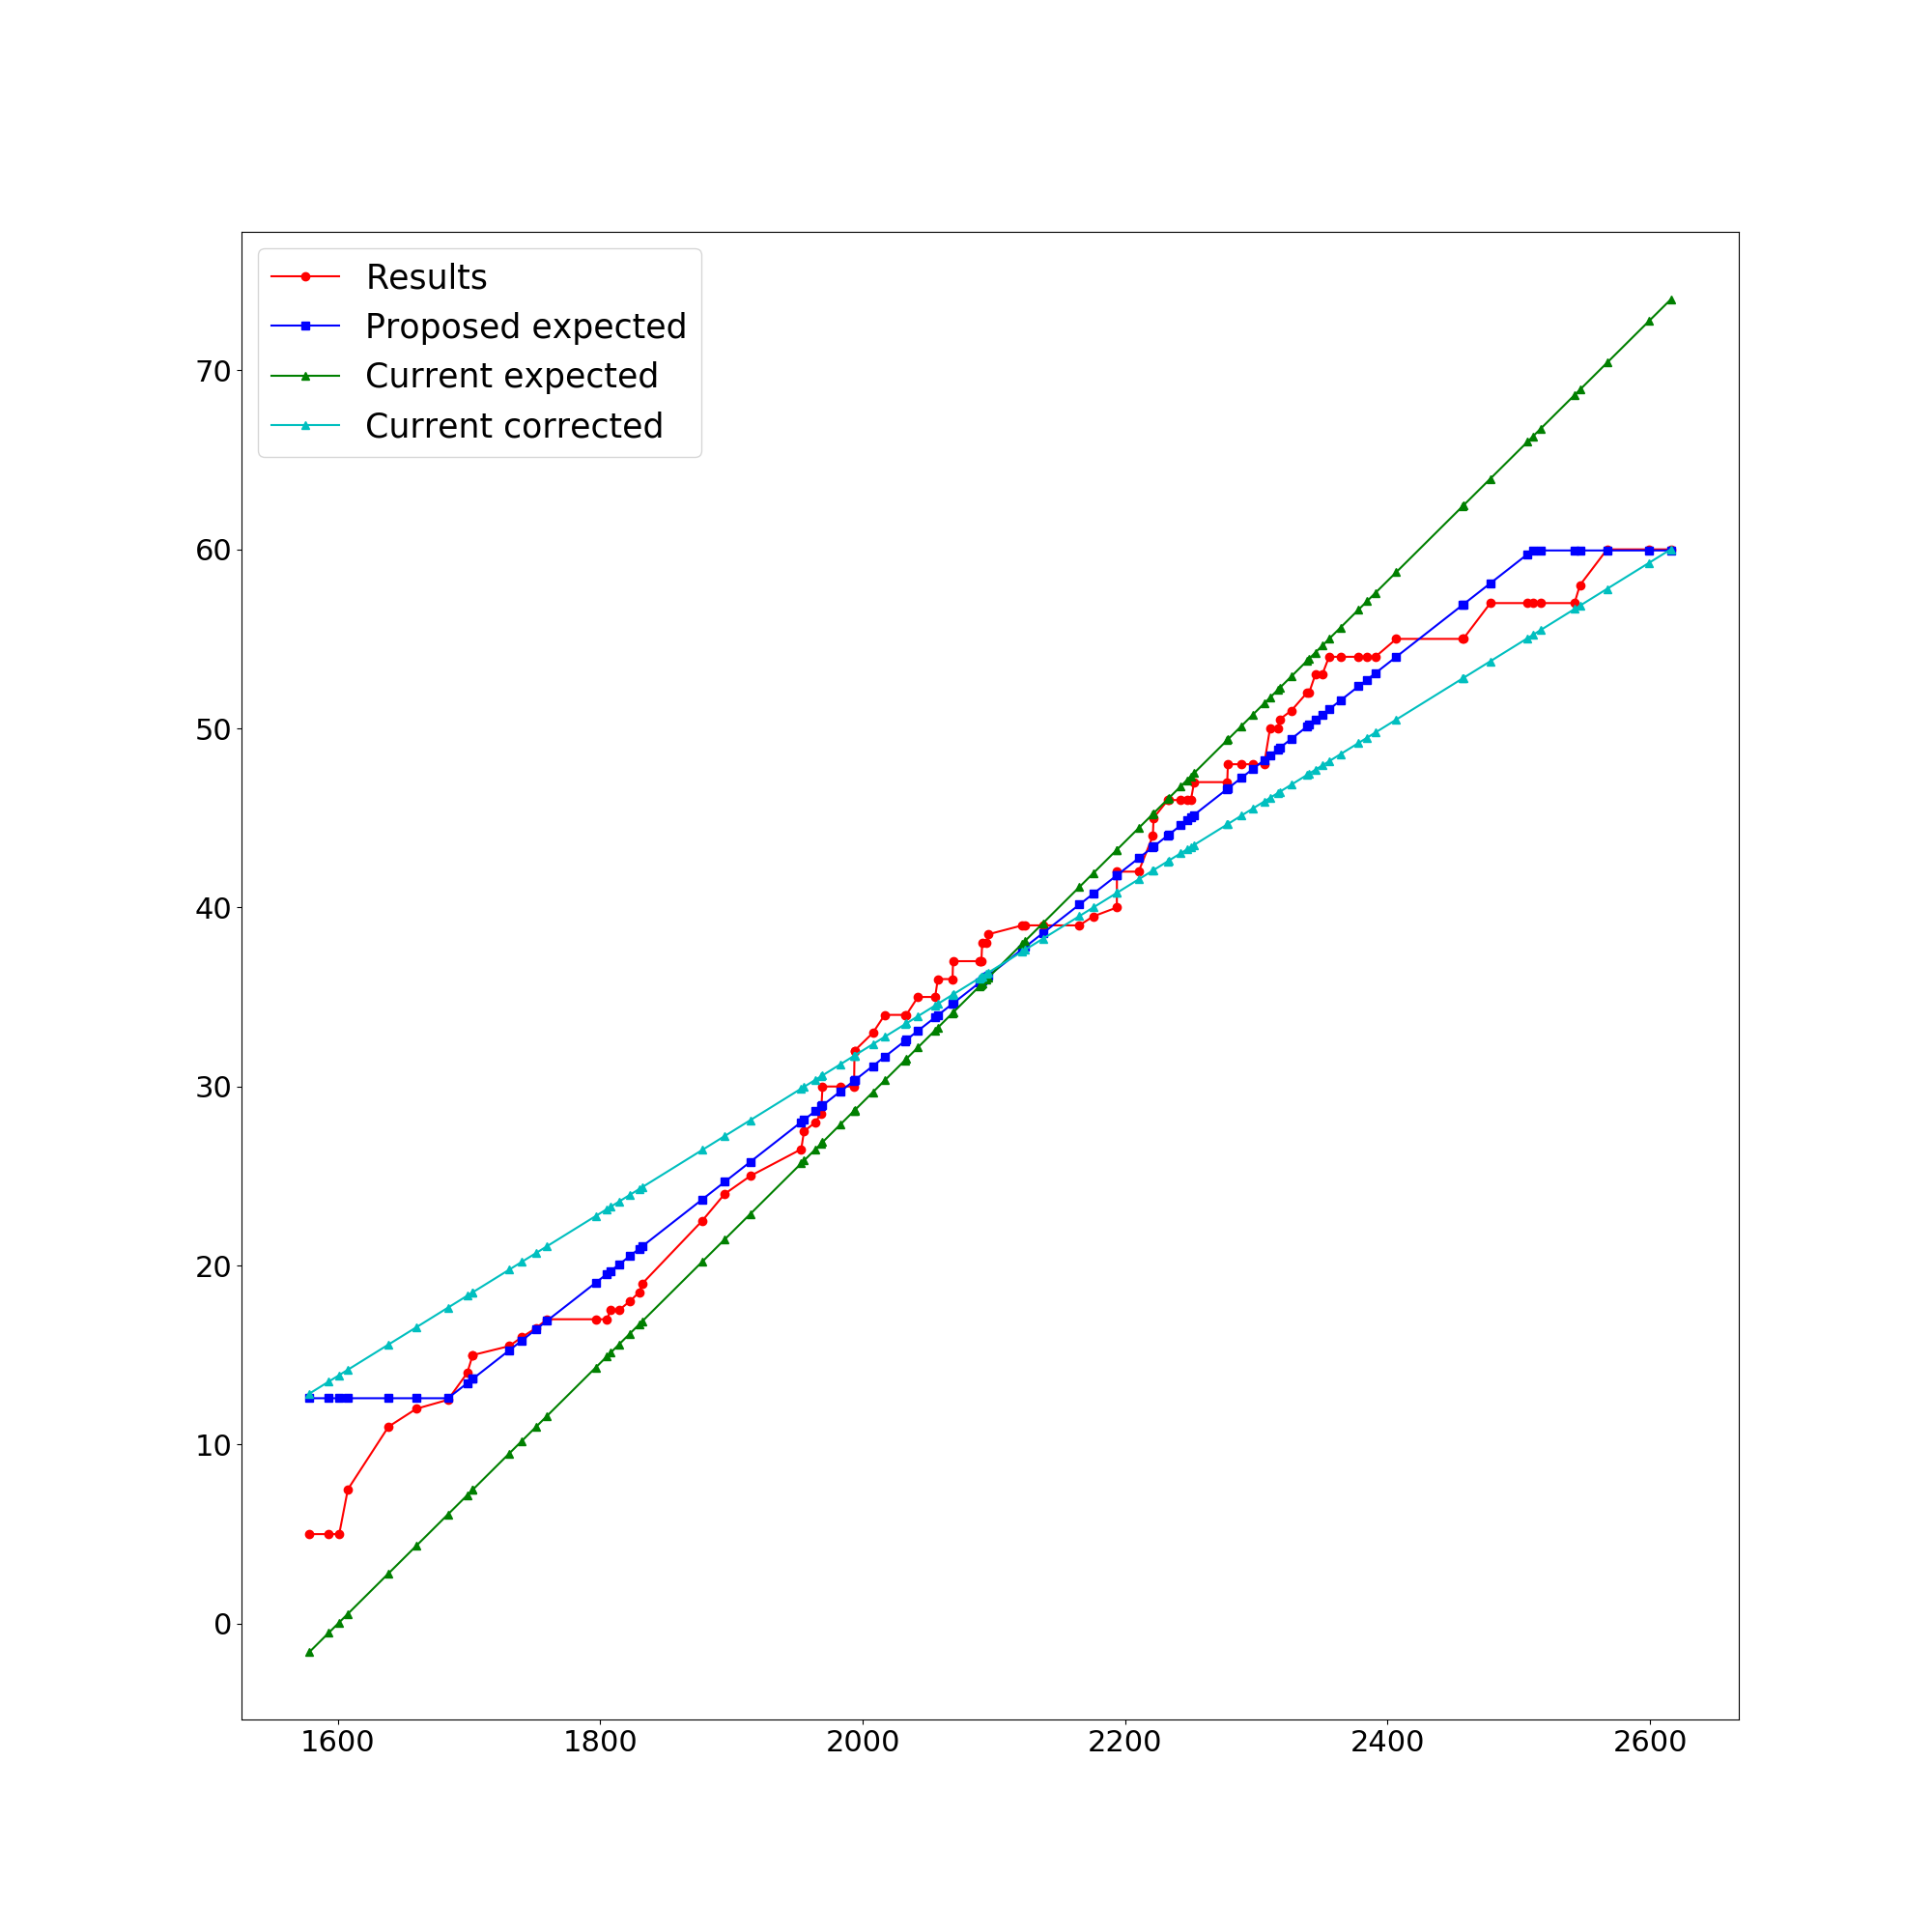
\includegraphics[width=1.0\linewidth]
{Israel_2017_points}\caption{Israel open 2017 points}
\label{israel_2017}
\end{figure}

\clearpage

\subsection{Numerical comparison}

Let $S'_i$ be the sorted array $S_i$,
and $R'_i$ be the sorted array $R_i$, both in non-decreasing order.
How could we compare quality of the proposed and the old system?
One reasonable way to measure it
is by calculating distance between projected scores and
points $(R'_i, S'_i)$ for $i\in\{1,\dots,n\}$ for arrays $R'$ and $S'$.

As a measure of distance of expected results $E_i$
and projected results $S'_i$
we take the mean square error ($\MSE$) for $i\in \{1,\dots,n\}$, that is:
\begin{equation}
\frac{1}{n}\sum_{i=1}^n (E_i-S'_i)^2,
\end{equation}
and mean absolute error ($\MAE$):
\begin{equation}
\frac{1}{n}\sum_{i=1}^n |E_i-S'_i|.
\end{equation}
After calculating these values for a couple
of last World Chess Solving Championship (WCSC),
as well as some recent open solving competitions,
we get results of MSE presented in Table~\ref{wcsc_mean_squared},
and results of MAE presented in Table~\ref{wcsc_mean_absolute}.

\begin{table}[h]
\begin{center}
\begin{tabular}{|c|c|c|c|}
\hline
Competition & $\MSE(\E)$ & $\MSE(\E')$ & $\MSE(E'')$\\
\hline
WCSC 2014 & $8.63$ & $17.67$ & $6.72$\\
\hline
WCSC 2015 & $8.58$ & & $7.86$\\
\hline
WCSC 2016 & $13.18$ & $2.98$ & $2.54$\\
\hline
WCSC 2017 & $7.25$ & & $4.54$\\
\hline
Israel open 2017 & $21.96$ & $13.00$ & $4.55$\\
\hline
Belgrade open 2018 & $9.16$ & & $3.68$\\
\hline
Warsaw open 2018 & $12.08$ & & $10.05$\\
\hline
\end{tabular}
\end{center}\caption{Mean Squared Error}\label{wcsc_mean_squared}
\end{table}

\begin{table}[h]
\begin{center}
\begin{tabular}{|c|c|c|c|}
\hline
Competition & $\MAE(\E)$ & $\MAE(\E')$ & $\MAE(E'')$\\
\hline
WCSC 2014 & $2.43$ & $3.70$ & $2.17$\\
\hline
WCSC 2015 & $2.25$ & & $2.11$\\
\hline
WCSC 2016 & $2.95$ & $1.19$ & $1.20$\\
\hline
WCSC 2017 & $1.87$ & & $1.51$\\
\hline
Israel open 2017 & $3.58$ & $3.00$ & $1.62$\\
\hline
Belgrade open 2018 & $2.38$ & & $1.41$\\
\hline
Warsaw open 2018 & $2.48$ & & $2.40$\\
\hline
\end{tabular}
\end{center}\caption{Mean Absolute Error}\label{wcsc_mean_absolute}
\end{table}

In all of the data presented in these two tables,
rating system proposed here gives at least as good,
and in most cases better estimations than the currently used one.

\end{document}
